\subsection{Peak Signal Noise Ratio}

The signal to noise ratio is a common tool to get an idea of how much signal is influenced by noise. It is calculated by weighing the power of the signal itself against the power of the noise.
\begin{align}
    SNR = \frac{P_{\text{Signal}}}{P_{\text{Noise}}}
\end{align}
As images can be seen as discrete signales in two dimensions this concept can also be applied to them. To avoid evaluating every pixel individually the peak signal to noise ratio (PSNR) can be used which repesents the maximum signal to noise ratio. In order to calculate the mean squared error (MSE) over the difference between the signal in question and the original image is needed. Typically the PSNR is calculated logarithmically to accommodate a wide range of MSEs.
\begin{align}
    PSNR = 10 * \log_10(\frac{R^2}{MSE}) [\mathrm{dB}]
\end{align}
As a general rule of thumb a higher PSNR means a better result and a better quality image.
A note for this implementation: When the MSE equates to zero $-1$ is returned as the PSNR would be $\infty$ which would make further calculations difficult.


\subsection{Monocular Depth Estimation} \label{mde_impl}

To lay a baseline for the accuracy of the GLPDepth we compared it to a ground truth and calculated the mean squared error (MSE) and peak signal to noise ratio (PSNR) in Dezibel. To do this we utilized svo files generated by a Stereolabs ZED2i stereo camera. Those files contain the video streams of both lenses, as well as of all other sensors. In our case the videostream had a resolution of 1920x1080 and was recorded with a framerate of 15fps.
The acompanying ZED SDK was used to calculate the depth images from that stereo camera setup as the ground truth. As will be discussed later, this is not necessarily optimal but sufficient.
The logged data gets temporarily stored in a numpy array and later written to an output csv file along with the frame index and time. The median and mean values over the aforementioned critical values get calculated just in time.


\subsection{Super Resolution}

The implementation is kept simple. Firstly we downscale the given raw images by x4 using the resize method of OpenCV. Then we load the pretrained model which can be obtained in the README of the ESRGAN \href{https://github.com/xinntao/ESRGAN}{repository} and tell the notebook to use the GPU and CUDA. After loading the model with the parameters, we apply it on the low resolution images. Lastly we calculate the PSNR by using the raw images and the results after the process.


\subsection{Combination}

\begin{figure}[ht!]
    \begin{center}
        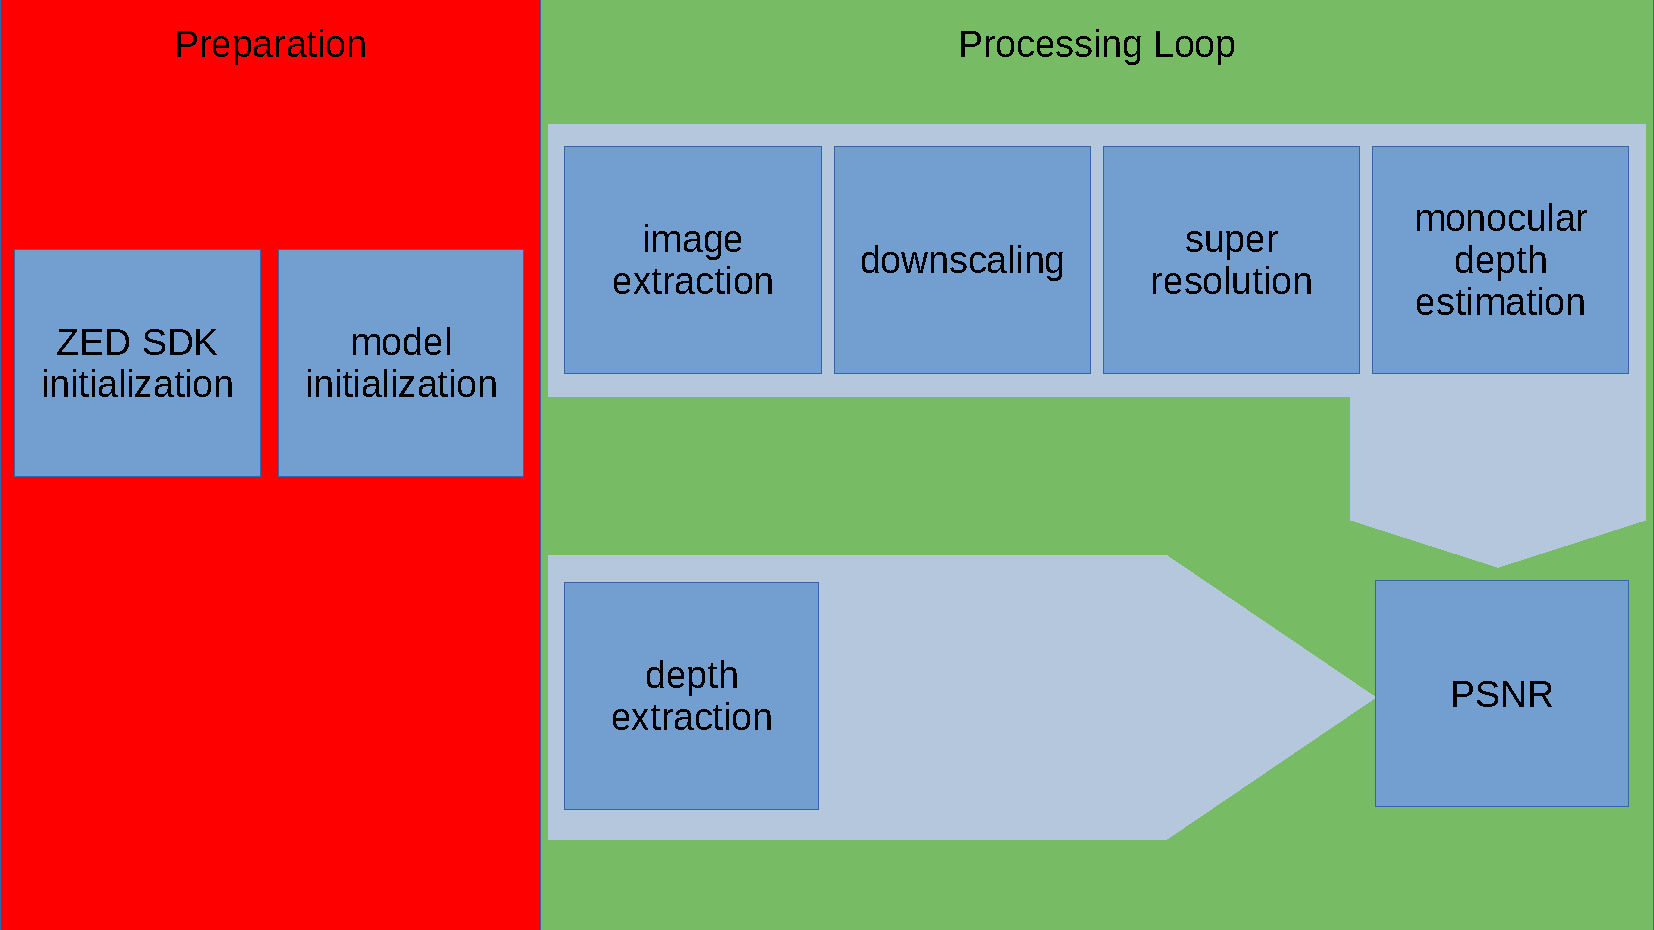
\includegraphics[scale=.5]{resources/general_plan.pdf}
        \caption{Flowchart of the final implementation.} \label{flowchart_general}
    \end{center}
\end{figure}

The actual implementation is very similar to the baseline implementation (Chapter \ref*{mde_impl}) in that there is a ground truth extracted from the given stereo information. But since the fine-grained information we would wish to extract with the super resolution is not available via this method the effect is approximated by first downscaling the left camera image by a factor of $4$ using OpenCV and subsequent upscaling via the super resolution model. This upscaled image is then used as input for the monocular depth estimation model to produce a depth image which in turn is compared against the ground truth. Again MSE and PSNR are used to determine the quality of the generated prediction. The time it took to process the images in the neural networks is also logged. Those evaluations are then stored and later saved to a csv file along with the mean and median values of the processing time, MSE and PSNR for evaluation.

The max depth is taken from the parameters used for the svo recording, which in this case is a range from $0.3\mathrm{m}$ to $20.0\mathrm{m}$. The initialization values for the GLPDepth model are taken from the implementation \href{https://github.com/vinvino02/GLPDepth}{repository} to accommodate the respective pretrained weights. The latter can also be downloaded as stated in the repositories README.

All images are cut or resized to a size of 1216x352 which is rather arbitrary and thus just adopted from the original implementation. This size could be some other size that fulfills the rule of being divisible by 4 in both directions. This constraint is necessary since the code does not explicitly check for mismatches between the ground truth and the resulting depth estimation resulting from a violation of this rule.

There are two pretrained weights available to choose from, which differentiate in the dataset used for training. One was trained on the KITTI Eigen Split while the other one was trained on Nyu Depth V2. These datasets are different from each other in the sense that the former covers primarily the outdoors while the latter contains inside references.
